Material
I virkeligheden har vi mange forskellige materialer der både syner og føles anderledes end andre. En helt ny bil skinner når man lyser på den, mens en murstensvæg er helt mat. For at illustrere det i raytracing har vi brugt nogen værdier der ofte bruges i forbindelse med 3D-rendering og især raytracing. Vi har valgt at bruge Phong-modellen da den er relativ simpel og giver et godt resultat.

\begin{lstlisting}[style=Cstyle, caption=Typedefinition af Material]
typedef struct _material {
  double ambient_coefficient;
  double diffuse_coefficient;
  double specular_coefficient;
  int smoothness;
  double metalness; 
} Material;
\end{lstlisting}

Ambient_coefficient er værdien der fortæller hvor lyst objektet er selvom der ikke er direkte lys på den. Den bevirker at hvis objektet er i skygge så er det ikke helt sort.
Diffuse_coefficient er skygge-værdien der viser hvor stor indflydelse lys har på objektet. 
Specular_coefficient er værdien der viser hvor meget objektet spejler igen. Denne værdi er høj for en ny poleret bil, men næsten 0 hvis det er en murstensvæg. I vores program gør det at vi får en næsten hvid plet hvis vores lyskilde spejler igen.

\begin{figure}[H]
    \centering
    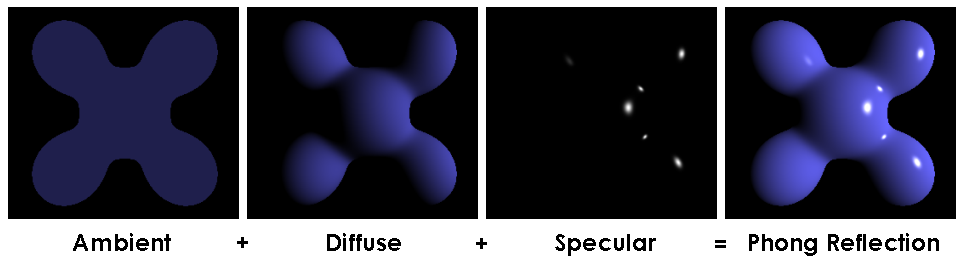
\includegraphics[width=10cm]{phong.png}
    \caption{Illustration af delene i phong-modellen}
    \label{fig:phong}
\end{figure} 
